\documentclass[12pt, a4paper]{article}
% Zobrazení frame - pro debug
%\usepackage{showframe}
% Tuto nechat
\usepackage{comment} 
\usepackage{lmodern}
\usepackage[inline]{enumitem}
\usepackage{xcolor}
\usepackage{blindtext}
\usepackage{scrextend}
\usepackage{cmap}
\usepackage[czech]{babel}
\usepackage[T1]{fontenc}
\usepackage[utf8]{inputenc}
\usepackage{graphicx}
\usepackage[capposition=bottom]{floatrow}
\usepackage{float}
\usepackage{amsmath}
\usepackage{pdfpages}
\usepackage{hyperref}
\addtokomafont{labelinglabel}
{\sffamily}
\begin{document}

% Pouze informace
\graphicspath{ {img/} }

% Úvodní stránka
\thispagestyle{empty}
\begin{center}
\begin{minipage}{0.75\linewidth}
    \centering
%University logo
    \vspace{3cm}
    
\includegraphics[width=0.75\linewidth]{fav-logo.pdf}\\
    \vspace{0.5cm}
%Thesis title
    {\uppercase{\Large KIV/PC \\ \textbf{Virtuální souborový systém založený na i-uzlech}\par}}
    \vspace{3cm}
%Author's name
    {\Large Jakub Vítek (viteja) - A19B0222P\par}
    \vspace{2cm}
%Degree
    \vspace{1cm}
%Date
    {\Large Leden 2020}
\end{minipage}
\end{center}
\clearpage
\newpage

% Část obsahu dokumentu
\tableofcontents
\newpage

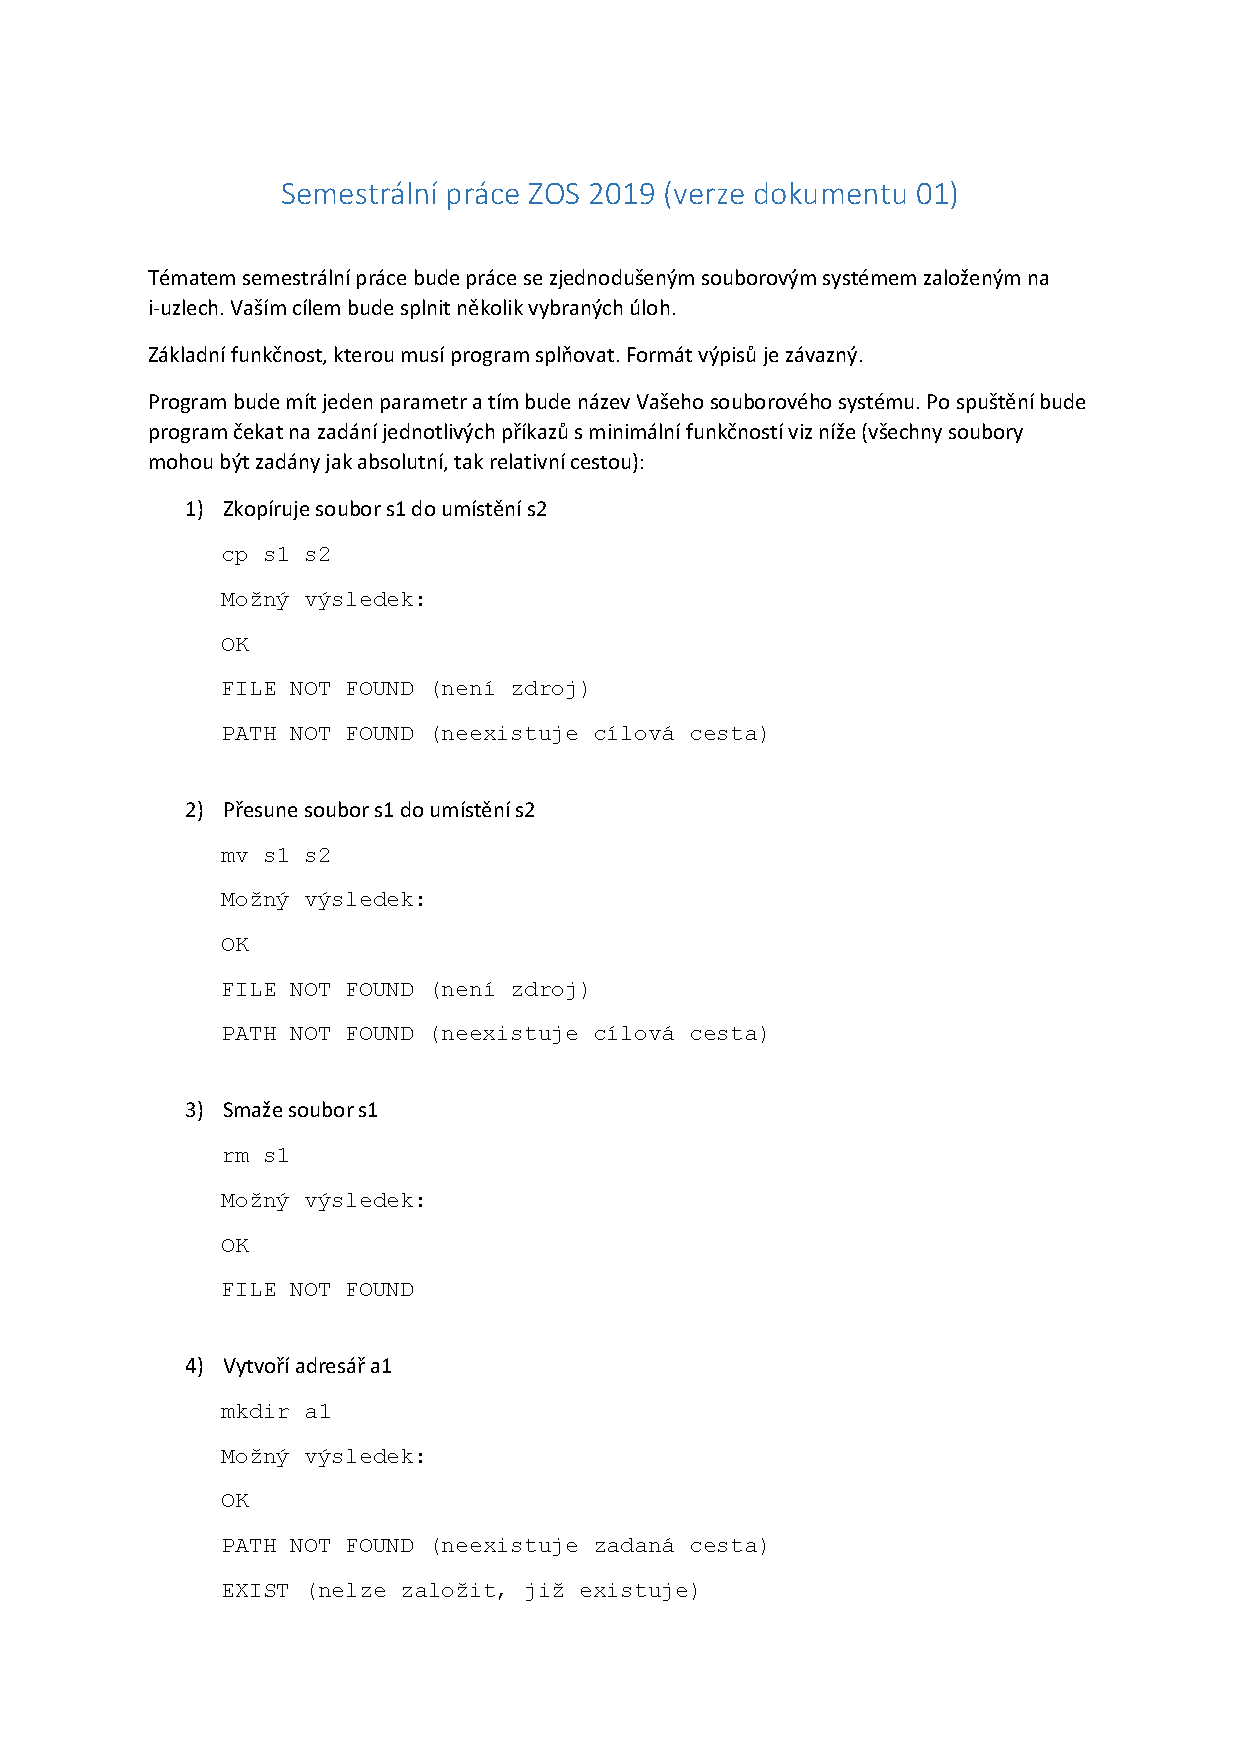
\includepdf[pages=-]{./include/zadani.pdf}

\section{Aplikace}
\paragraph{}
Aplikace byla primárně vyvíjena, ve standardu C99 programovacího jazyka C, pro operační systém GNU/Linux (Fedora 31), měla by však podporovat všechny operační systémy podporující standard POSIX. Pro kompatibilitu s operačním systémem Windows byla část zdrojového kódu reimplementována či nahrazena, kompatibilita je docílena využitím podmínek a maker preprocessoru jazyka C. 

\paragraph{}
Aplikace má několik základních omezení v parametrech. Některá omezení jsou umělá, například dodržení maximální velikosti souboru 12 byte, spousta omezení však vyplývá z implementace aplikace za pomocí 32 bitových hodnot. Zbylé hodnoty by mohly být měnitelné (například velikost datového bloku), byly však pěvně implementované. 

\paragraph{}
Program je spustitelným binárním souborem, který má jeden povinný vstupní parametr - cestu k virtuálnímu souborovému systému (VFS). V případě, že existuje rodičovská složka a neexistuje soubor VFS, soubor bude vytvořen a naformátován na velikost 64kB.

\paragraph{}

\newpage
\section{Struktura}
\paragraph{}
Struktura souboru je závislá na požadované velikosti.

\subsection{Superblok}
Virtuální souborový systém obsahuje jeden superblok, který je umístěn v hlavičce na začátku souboru VFS a jeho velikost je 284 byte. Tato struktura obsahuje základní informace o umístění jednotlivých částí VFS. Defici struktury lze vidět v hlavičkovém souboru \textit{superblock.h}.

\subsection{Hlavička a datová část}
Velikost hlavičky souborového systému se odvíjí od celkové velikosti souboru. Na hlavičku jsou pevně vyhrazená 4\% celkové velikosti systému (např. 600MB soubor => 600MB * 4\% = 24MB). Hlavička obsahuje (v tomto pořadí): \textit{superblok}, \textit{bitmapu}, \textit{prostor pro i-uzly}. Formátování souborového systému proběhne úspěšně i v případě, že prostor pro hlavičku je příliš malý, například když se nezapíše dostatečné množství byte pro bitmapu či pro i-uzly. Takto malé systémy jsou však nepoužitelné. Zbylých 96\% je využito pro ukládání dat. 

\subsection{Bitmapa}
Bitmapa je součástí hlavičky souborového systému a její velikost je na celkové velikosti VFS závislá. Jeden blok bitmapy je velký 1 byte a může obsahovat hodnotu 0 (indikace volného databloku), hodnotu 1 (indikace využitého databloku) či jinou chybovou hodnotu. Počet bloků bitmapy je při dostatku místa pro VFS celkovým počtem datových bloků. 

\subsection{I-uzly}   
Po té, co do vyhrazených 4\% hlavičky VFS jsou zapsány superblok a bitmapa, je zbylé volné místo využito na uložení i-uzlu. Samotný i-uzel má 44 Byte, některé ukazatele jsou však uloženy do datových bloků jako první či druhý nepřímý ukazatel. Na obsah virtuálního souborového systému je od počáteční adresy pro i-uzly do počátku datové části nahlíženo jako na pole. I-uzly jsou číslovány dle jejich pořadí zápisu. 

\subsection{Datová část}
Zbylá část virtuálního souborového systému obsahuje místo, pro uložení dat. Toto místo je rozděleno na datové bloky. Jeden datový blok má v současné implementaci velikost 4096 byte. Indikace, zda je datový blok využíván, je umístěna v bitové mapě. Nultý datový blok je nultým blokem bitmapy. 

\newpage
\section{Input/Output}
\paragraph{}
Virtuální souborový systém v rámci této aplikace je standardním souborem na hostitelském operačním systému (GNU/Linux, Windows), který dodržuje strukturu popsanou v předchozí kapitole. Aplikace vnitřně pro všechny úpravy používá knihovnu \textit{stdio.h} (funkce fopen, fseek, fwrite, fread, fclose). Vzhledem k tomu, že nahrávané soubory nemusí být umístěny kontiunálně na sobě navazujících datových blocích, bylo třeba přístup k datům standardizovat, jinak by zdrojový kód pro práci s vnitřními VFS soubory byl extrémně opakován a zvyšoval nečitelnost.    
  
\paragraph{}
Z tohoto důvodu byla provedena zjednodušená reimplementace výše uvedených funkcí - \textit{VFS\_IO.h} (VFS\_FILE, VFS\_open, VFS\_seek, VFS\_read, VFS\_write, VFS\_close). Tato miniknihovna umožnuje pracovat s vnitřním souborem VFS dostatečně podobným způsobem jako v případě stdio.h. 

\newpage
\section{Soubory}
\paragraph{}
V tomto virtuálním souborovém systému platí, že jeden i-uzel se rovná jednomu souboru bez ohledu na typ souboru. Každý soubor má přiděleny přímé či nepřímé datové bloky, které určují jeho prostor pro čtení a zápis dat. Soubory se virtuálně 

Souborový systém má tři základní typy souborů. 

\subsection{Soubor} 
\paragraph{}
Obyčejný binární soubor bez speciálně definované struktury. 

\subsection{Složka}
\paragraph{}
Složka je souborem. Každých 16 byte tohoto souboru lze převést na data struktury \textit{directory\_entry}. Každá složka má minimálně dvě tyto struktury, což znamená, že minimální velikost složky je 32 byte. První dvě struktury obsahují: záznam pro aktuální složku a záznam rodičovské složky. 
\paragraph{}
Složky virtuálně vytváří stromovou strukturu, která začíná kořenovou složkou, která má ID = 1 a první dva záznamy ve složce stejné. 


\subsection{Symbolický link}
\paragraph{}
Symbolický link je soubor obsahující řetězec, který je cestou k souboru, na který symbolický link ukazuje. 


\newpage
\section{Příkazový řádek}
\paragraph{}
Příkazový řádek dovoluje interakci uživatele s virtuálním souborovým systémem. Příkazový řádek je cyklem, který vypíše cestu složku, do které je uživatel právě přepnut (před znakem \textit{>}). Následně je očekáván vstup od uživatele (jeden z příkazů uvedených v zadání). Vstup je zpracován a probíhá ověření, jestli se nejedná o rozpoznaný příkaz. V případě, že je příkaz rozpoznán, zpracovaný vstup od uživatele je předán funkci, která ověří požadované parametry a provede akci. 

\ paragraph{}
Seznam příkazů lze vidět v zadání práce. K těmto příkazům byl navíc doplněn příkaz exit, jež bezpečně ukončí program (ukončení lze také provést zkratkou ctrl+c [SIGINT] ve chvíli kdy příkazový řádek čeká na vstup) 

\newpage
\section{Uživatelská příručka}
\subsection{Překlad a sestavení}
\paragraph{}
Aplikaci lze přeložit, sestavit a spustit pod operačními systémy GNU/Linux (instalujte: gcc, make dle pokynů Vaší distribuce) a Windows (instalujte: MinGW - gcc, make). \\ Aplikaci je doporučeno sestavit přiloženými Makefile (Makefile.win pro windows). 

\subsection{Spuštění}
\paragraph{}
Po překladu a sestavení pomocí přiložených makefile lze aplikaci spustit příkazem \verb|./KIV_ZOS <cesta_k_vfs_souboru>|. Parametr aplikace je povinný. Cesta k rodičovské složce VFS souboru musí existovat, soubor samotný nikoliv - v případě, že soubor neexistuje, bude vytvořen a naformátován na velikost 64KB.

\subsection{Ovládání}
\paragraph{}
Aplikace žádá od uživatele vstupní příkazy v podobném duchu jako při práci se soubory v operačním systému GNU/Linux. Seznam příkazů je možné přečíst v zadání práce. 


\newpage
\section{Závěr}
\paragraph{}
Implementoval jsem relativně komplexní aplikaci (na poměry toho, co se obvykle dělá v předchozích předmětech na FAV ZČU). Aplikaci jsem primárně vyvíjel a testoval na operačním systému GNU/Linux s podporou a testováním na systému Microsoft Windows. 
\paragraph{}
Aplikace má mnoho nedostatků, při vývoji jsem bohužel zvolil 32 bitová čísla, jež mě značně omezují. Dále jsem při vývoji zahodil možnost rozsáhlejší nastavitelnosti programu (např. velikost datového bloku). Aplikace striktně běží na jediném vláknu, čtení a zápis nemají svou vyrovnávací pamět, takže se rychlost aplikace zpomaluje čekáním na I/O operace.
\paragraph{}
I přes tyto nedostatky však aplikace splňuje všechny požadavky. 



\end{document}